\documentclass[table]{beamer}
%[]中可以使用draft、handout、screen、transparency、trancompress、compress等参数

%指定beamer的模式与主题
\mode<presentation>
{
  \usetheme{Madrid}
%\usetheme{Boadilla}
%\usecolortheme{default}
%\usecolortheme{orchid}
%\usecolortheme{whale}
%\usefonttheme{professionalfonts}
}

%\usetheme{Madrid}
%这里还可以选择别的主题:Bergen, Boadilla, Madrid, AnnArbor, CambridgeUS, Pittsburgh, Rochester, Warsaw, ...
%有导航栏的Antibes, JuanLesPins, Montpellier, ...
%有内容的Berkeley, PaloAlto, Goettingen, Marburg, Hannover, ...
%有最小导航栏的Berlin, Ilmenau, Dresden, Darmstadt, Frankfurt, Singapore, Szeged, ...
%有章和节表单的Copenhagen, Luebeck, Malmoe, Warsaw, ...

%\usecolortheme{default}
%设置内部颜色主题(这些主题一般改变block里的颜色);这个主题一般选择动物来命名
%这里还可以选择别的颜色主题,如默认的和有特别目的的颜色主题default,structure,sidebartab,全颜色主题albatross,beetle,crane,dove,fly,seagull,wolverine,beaver

%\usecolortheme{orchid}
%设置外部颜色主题(这些主题一般改变title里的颜色);这个主题一般选择植物来命名
%这里还可以选择别的颜色主题,如默认的和有特别目的的颜色主题lily,orchid,rose

%\usecolortheme{whale}
%设置字体主题;这个主题一般选择海洋动物来命名
%这里还可以选择别的颜色主题,如默认的和有特别目的的颜色主题whale,seahorse,dolphin

%\usefonttheme{professionalfonts}
%类似的还可以定义structurebold,structuresmallcapsserif,professionalfonts

% 控制 beamer 的风格,可以根据自己的爱好修改
%\usepackage{beamerthemesplit} %使用 split 风格
%\usepackage{beamerthemeshadow} %使用 shadow 风格
%\usepackage[width=2cm,dark,tab]{beamerthemesidebar}

%插入音标
%\usepackage{tipa}
%\AtBeginDocument{
  %\renewcommand\textipa{\fontencoding{T3}\selectfont}
%}
%\AtBeginDocument{
  %\renewcommand\textipa[2][r]{{\fontfamily{cm#1}\tipaencoding #2}}
%}
%\renewenvironment{IPA}[1][r]
 %{\fontfamily{cm#1}\tipaencoding}
 %{}

% 设定英文字体
%\usepackage{fontspec}
% Fix bugs for fontspec in TeXLive2015
\ifdefined\suppressfontnotfounderror
  \expandafter\let\csname xetex_suppressfontnotfounderror:D\endcsname
    \suppressfontnotfounderror
\else
  \expandafter\let\csname xetex_suppressfontnotfounderror:D\endcsname
    \luatexsuppressfontnotfounderror
\fi
\usepackage[no-math]{fontspec}
\setmainfont{Times New Roman}
\setsansfont{Arial}
\setmonofont{Courier New}

% 设定中文字体
\usepackage[BoldFont,SlantFont,CJKchecksingle,CJKnumber]{xeCJK}
%\setCJKmainfont[BoldFont={Adobe Heiti Std},ItalicFont={Adobe Kaiti Std}]{Adobe Song Std}
\setCJKmainfont[BoldFont={Adobe Heiti Std},ItalicFont={Adobe Kaiti Std}]{WenQuanYi Micro Hei}
\setCJKsansfont{Adobe Heiti Std}
\setCJKmonofont{Adobe Fangsong Std}
\punctstyle{hangmobanjiao}

\defaultfontfeatures{Mapping=tex-text}
\usepackage{xunicode}
\usepackage{xltxtra}

\XeTeXlinebreaklocale "zh"
\XeTeXlinebreakskip = 0pt plus 1pt minus 0.1pt

\usepackage{setspace}
\usepackage{colortbl,xcolor}
\usepackage{hyperref}
%\hypersetup{xetex,bookmarksnumbered=true,bookmarksopen=true,pdfborder=1,breaklinks,colorlinks,linkcolor=blue,filecolor=black,urlcolor=cyan,citecolor=green}
\hypersetup{xetex,bookmarksnumbered=true,bookmarksopen=true,pdfborder=1,breaklinks,colorlinks,linkcolor=cyan,filecolor=black,urlcolor=blue,citecolor=green}

% 插入图片
\usepackage{graphicx}
\graphicspath{{figures/}}
% 图文混排
%\usepackage{picins}
\usepackage{floatflt}

% 可能用到的包
\usepackage{amsmath,amssymb}
%插入多媒体
%\usepackage{media9}
%\usepackage{movie15}
\usepackage{multimedia}
\usepackage{multicol}
\usepackage{multirow}

% 定义一些自选的模板,包括背景、图标、导航条和页脚等,修改要慎重
% 设置背景渐变由10%的红变成10%的结构颜色
%\beamertemplateshadingbackground{red!10}{structure!10}
%\beamertemplatesolidbackgroundcolor{white!90!blue}
% 使所有隐藏的文本完全透明、动态,而且动态的范围很小
\beamertemplatetransparentcovereddynamic
% 使itemize环境中变成小球,这是一种视觉效果
\beamertemplateballitem
% 为所有已编号的部分设置一个章节目录,并且编号显示成小球
\beamertemplatenumberedballsectiontoc
% 将每一页的要素的要素名设成加粗字体
\beamertemplateboldpartpage

% item逐步显示时,使已经出现的item、正在显示的item、将要出现的item呈现不同颜色
\def\hilite<#1>{
 \temporal<#1>{\color{gray}}{\color{blue}}
    {\color{blue!25}}
}

\renewcommand{\today}{\number\year 年 \number\month 月 \number\day 日}

%五角星
\usepackage{MnSymbol}

%去除图表标题中的figure等
\usepackage{caption}
\captionsetup{labelformat=empty,labelsep=none}

\usepackage{tabu}
\usepackage{multirow}
%表格自动换行
\usepackage{tabularx} 

% 千分号
%\usepackage{textcomp}

%罗马数字
\makeatletter
\newcommand{\rmnum}[1]{\romannumeral #1}
\newcommand{\Rmnum}[1]{\expandafter\@slowromancap\romannumeral #1@}
\makeatother

%分栏
\usepackage{multicol}

%\usepackage{enumitem}
%\usepackage{enumerate}

%键盘
\usepackage{keystroke}

%心形
%\usepackage{fdsymbol}

%插入源代码
\usepackage{listings}
\lstset{
  language=perl,                  % 程序语言名称:TeX, Perl, R, sh, bash, Awk
  basicstyle=\normalsize\tt,      %\tt指monospace字体族,程序源代码使用此族字体表示更加美观
  numbers=left,                   % 行号位置(左侧)
  numberstyle=\small,             % 行号字体的字号
  stepnumber=1,                   % 行号的显示步长
  numbersep=5pt,                  % 行号与代码间距
  backgroundcolor=\color{white},  % 背景色;需要 \usepackage{color}
  showspaces=false,               % 不显示空格
  showstringspaces=false,         % 不显示代码字符串中的空格标记
  showtabs=false,                 % 不显示 TAB
  tabsize=4, 
  frame=shadowbox,                % 把代码用带有阴影的框圈起来
  captionpos=b,                   % 标题位置
  breaklines=true,                % 对过长的代码自动断行
  breakatwhitespace=false,        % 断行只在空格处
  extendedchars=false,            % 解决代码跨页时,章节标题,页眉等汉字不显示的问题
  %escapeinside={\%*}{*},         % 跳脱字符,添加注释,暂时离开 listings 
  %escapeinside=``,
  commentstyle=\color{red!50!green!50!blue!50}\tt,  %浅灰色的注释
  rulesepcolor=\color{red!20!green!20!blue!20},     %代码块边框为淡青色
  keywordstyle=\color{blue!70}\bfseries\tt,         %代码关键字的颜色为蓝色,粗体
  identifierstyle=\tt,
  stringstyle=\tt,                % 代码字符串的特殊格式
  keepspaces=true,
  breakindent=1em,
  %breakindent=22pt,
  %breakindent=4em,
  breakautoindent=true,
  flexiblecolumns=true,
  aboveskip=1em,                  %代码块边框
  xleftmargin=2em,
  xrightmargin=2em
}

%\setbeamercolor{alerted text}{fg=magenta}
\setbeamercolor{bgcolor}{fg=yellow,bg=cyan}
%\setbeamercolor{itemize/enumerate body}{fg=green}

\begin{document}

%\includeonlyframes{current}

\logo{
\includegraphics[height=0.08\textwidth]{qr.png}}

% 在每个Section前都会加入的Frame
\AtBeginSection[]
{
  \begin{frame}<beamer>
    %\frametitle{Outline}
    \frametitle{教学提纲}
    \setcounter{tocdepth}{3}
    \begin{multicols}{2}
      \tableofcontents[currentsection,currentsubsection]
      %\tableofcontents[currentsection]
    \end{multicols}
  \end{frame}
}
% 在每个Subsection前都会加入的Frame
\AtBeginSubsection[]
{
  \begin{frame}<beamer>
%%\begin{frame}<handout:0>
%% handout:0 表示只在手稿中出现
    \frametitle{教学提纲}
    \setcounter{tocdepth}{3}
    \begin{multicols}{2}
    \tableofcontents[currentsection,currentsubsection]
    \end{multicols}
%% 显示在目录中加亮的当前章节
  \end{frame}
}

% 为当前幻灯片设置背景
%{
%\usebackgroundtemplate{
%\vbox to \paperheight{\vfil\hbox to
%\paperwidth{\hfil\includegraphics[width=2in]{tijmu_charcoal.png}\hfil}\vfil}
%}
\begin{frame}[plain]
  \begin{center}
    {\Huge 故事中的统计学\\}
    \vspace{1cm}
    {\LARGE 天津医科大学\\}
    %\vspace{0.2cm}
    {\LARGE 生物医学工程与技术学院\\}
    \vspace{1cm}
    {\large 2017-2018学年下学期(春)\\ 公共选修课}
  \end{center}
\end{frame}
%}



%\includeonlyframes{current}

\title[抽样]{第一章\quad 内在有偏的样本}
\author[Yixf]{伊现富(Yi Xianfu)}
\institute[TIJMU]{天津医科大学(TIJMU)\\ 生物医学工程与技术学院}
\date{2017年4月}

\begin{frame}
  \titlepage
\end{frame}

\begin{frame}[plain,label=current]
  \frametitle{教学提纲}
  \setcounter{tocdepth}{3}
  \begin{multicols}{2}
    \tableofcontents
  \end{multicols}
\end{frame}


\section{抽样}
\begin{frame}
  \frametitle{抽样 | 简介}
  \begin{block}{双色豆子}
    有一个装着红、白两色豆子的桶,如果想知道桶中两种豆子的数量:
    \begin{itemize}
      \item 准确知道 $\Longrightarrow$ 一颗一颗地数豆子
      \item 粗略估计 $\Longrightarrow$ 抓一把豆子数一数
    \end{itemize}
  \end{block}
  \pause
  \begin{figure}
    \centering
    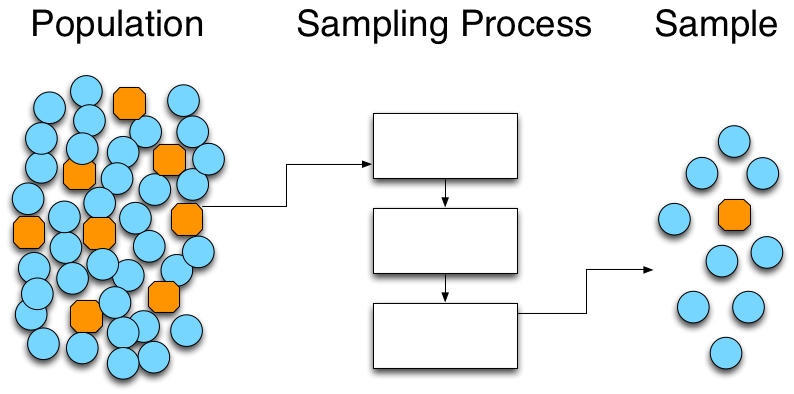
\includegraphics[width=0.8\textwidth]{c1.sampling.01.png}
  \end{figure}
\end{frame}

\begin{frame}
  \frametitle{抽样 | 简介}
  \begin{block}{生活实例}
    \begin{itemize}
      \item 从一锅汤里舀出一勺进行品尝,从而知道整锅汤的味道
      \item 从一锅水饺里面捡出一个尝一下,从而确定水饺熟没熟
      \item 交通警察抽取司机的血液来确定酒精含量(各种抽血、验尿检查)
    \end{itemize}
  \end{block}
  \pause
  \begin{block}{前提}
    \begin{itemize}
      \item 样本足够大
      \item 选择样本的方法正确
    \end{itemize}
  \end{block}
\end{frame}

\begin{frame}
  \frametitle{抽样 | 总结}
  \begin{block}{总结}
如果样本足够大,并且选择方法正确,在大多数情况下它能够很好地代表整体。但是,如果以上两个条件不满足,这样的样本比一个臆想好不到哪儿去。不幸的是,我们所看到的,或者我们自以为了解的许多事物,往往都是根据类似样本所得出的结论,这种样本可能变得有偏,由于选择方式的不合理或者容量过小,抑或两种情况同时存在。
  \end{block}
  \pause
  \begin{block}{应用}
很少有人知道,公开数据其实是来自样本。国家统计局的网站首页,刊登了各式各样有关于经济、人口及社会的数据,其实这些数据几乎都是根据抽样结果推算出来的。
  \end{block}
\end{frame}

\section{案例分析}
\subsection{选择性偏见}
\begin{frame}
  \frametitle{案例分析 | 选择性偏见}
  \begin{block}{生活实例}
    \begin{itemize}
      \item “尼克松/特朗普不可能赢,我认识的人都没有投票给他。”
      \item “中医真厉害/都是骗人的,我认识的人生病都吃中药吃好了/一点用也没有。”
    \end{itemize}
  \end{block}
  \pause
  \begin{block}{一个我们应该经常问自己的问题}
    在给出评价之前,我们是如何选择样本的?如果人口中的每一个人被选入样本的概率不是均等的,那么由这样一个样本推导出的结论就会存在问题。
  \end{block}
\end{frame}

\begin{frame}
  \frametitle{案例分析 | 选择性偏见 | 预测美国大选}
  \begin{block}{1936年《文学文摘》的民意测验}
    1936年,共和党人兰登和民主党人罗斯福竞选美国总统。《文学文摘》向该杂志的订阅者以及能够从公共档案中查到地址的汽车和电话主人寄去了一份调查问卷,总共加起来有1000万名美国公民收到了这份问卷,这个样本容量在当时算得上是天文数字了。《文学文摘》预测兰登将以57\%的支持率击败罗斯福赢得选举。而事实是,罗斯福获得了60\%的选民投票以及多达46个州(总共48个州)的支持,以压倒性优势赢得了选举。
%曾经准确预测了1932年美国大选的1000万个电话用户和《文学文摘》订户,又对1936年的大选结果进行了预测,他们信誓旦旦地保证:兰登将在竞选中脱颖而出,并且与罗斯福的所得票数之比为370:161。
  \end{block}
  \pause \pause \pause \pause
  \begin{block}{解析}
    该杂志的订阅者们比普通美国人要富有,因此更有可能投票给保护富人利益的共和党,1936年家中就拥有汽车和电话的选民的投票情况也是如此。
% 1936年就有能力购买电话和订阅杂志的人并不能代表所有的选民,至少在经济上,他们是一个极特殊的群体,是有偏的。(后来证实他们中的许多人是共和党的选民。)
  \end{block}
\end{frame}

\begin{frame}
  \frametitle{案例分析 | 选择性偏见 | 前列腺癌治疗的副作用}
  \begin{block}{短程疗法对男性性功能损伤最小?}
    \begin{itemize}
      \item 背景:
通常针对前列腺癌患者有3种治疗方法:手术移除前列腺、放射治疗、短程疗法(将放射性“种子”植入癌细胞集中区域)。阳痿是前列腺癌治疗最常见的副作用。
      \item 数据: 在接受治疗的两年之后,一项针对1000名男性的调查结果发现,手术移除组有35\%的男性能够进行性生活;放射组能进行性生活的男性占37\%;在接受短程疗法的男性患者中,有43\%的人恢复了性生活。
    \end{itemize}
  \end{block}
  \pause \pause \pause \pause
  \begin{block}{解析}
    由于接受短程疗法的患者通常较为年轻,健康状况也比接受另外两种疗法的病人要好,因为不能得出短程疗法对男性性功能损伤最小的结论。
  \end{block}
\end{frame}

\begin{frame}
  \frametitle{案例分析 | 选择性偏见 | CA125水平与卵巢癌}
  \begin{block}{检测CA125蛋白在血液中的水平推断患者是否可能会患有卵巢癌}
    开发这种筛查的实验室声称卵巢癌检查的PPV(阳性预测值,positive predictive value)为99.3\%,拥有很高的检出率。
  \end{block}
  \pause \pause \pause \pause
  \vspace{-0.3em}
  \begin{block}{解析(FDA认定筛查这种蛋白质不能提供明确的作用)}
    这个数字是基于一项单一无对比的实验得出的,实验中有半数患者已经确诊患有卵巢癌了——这是一个经过高度选择的人群。
  \end{block}
  \pause \pause \pause \pause
  \vspace{-0.3em}
  \begin{block}{类比——因?果?}
    如果你把挂了鱼饵的鱼钩投入一个装满鱼的桶中,当你感觉鱼线被拖拽时,有鱼上钩的可能性非常大。不过,如果这个挂了饵的鱼钩投入的是一个没有鱼的淡水湖,鱼线拖拽时,有鱼上钩的可能性就低了很多,更有可能的是被树杈挂住了。因为相同体积的水里,桶里的鱼比湖里要多得多,所以桶里的拖拽PPV接近100\%,而没有鱼的湖里,拖拽PPV要低很多。
  \end{block}
\end{frame}

\begin{frame}
  \frametitle{案例分析 | 选择性偏见 | 留学生与本地学生}
  \begin{block}{亚洲留学生更聪明}
    外国留学生尤其是来自中国内地和中国香港的留学生,通常要比加拿大的学生表现得更加聪明、好学、成绩优秀。他们没有一个不及格,然而相比而言,当地加拿大学生中有1/3没有通过课程。
  \end{block}
  \pause \pause \pause \pause
  \begin{block}{解析}
    只有实际上真正聪明的、有才智的好学生才被送到海外读书。用优秀的群体与加拿大普通的学生之间进行比较,其结果可想而知。
  \end{block}
\end{frame}

\begin{frame}
  \frametitle{案例分析 | 选择性偏见 | 其他}
  \begin{block}{选择性偏见}
    \begin{itemize}
      \item 针对某一机场消费者展开的调查
      \item 在州际公路旁的一个休息点展开的调查
      \item 在一个公共场合询问100个人是否愿意接受一个小调查
      \item 国内外教材的对比:国外教材深入浅出、都是经典,国内教材东拼西凑、一堆垃圾
      \item 戒毒组的成员在出狱之后再次入狱的概率要比没有参加戒毒组的犯人小
      \item 孕妇在家中生产肯定会比在医院更加安全一些
      \item “试管婴儿”出生时的死亡率是其他婴儿的3倍多
    \end{itemize}
  \end{block}
\end{frame}

\begin{frame}
  \frametitle{案例分析 | 选择性偏见 | 其他}
  \begin{block}{选择性偏见}
    \begin{itemize}
      \item 广播、电视、报纸上的各种报道(中央领导很忙,中国人民很幸福,世界人民生活在水深火热之中——《新闻联播》)
      \item 《全民目击》(Silent Witness)
    \end{itemize}
    \vspace{-1em}
    \begin{figure}
      \centering
      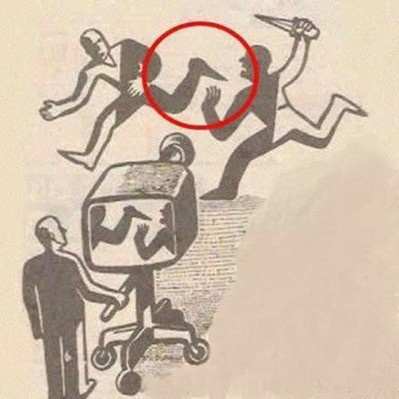
\includegraphics[width=0.5\textwidth]{c1.news.01.jpg}
    \end{figure}
  \end{block}
\end{frame}

\subsection{幸存者偏见}
\begin{frame}
  \frametitle{案例分析 | 幸存者偏见 | 为轰炸机增加装甲防护}
  \begin{block}{轰炸机}
在二战中,美国人曾经研究了他们的轰炸机如何才能避开德国的防空炮火而击中目标:轰炸机的哪一部分最经常被敌机击中,在飞机的什么部位增加装甲防护是必要的?
  \end{block}
  \begin{figure}
    \centering
    %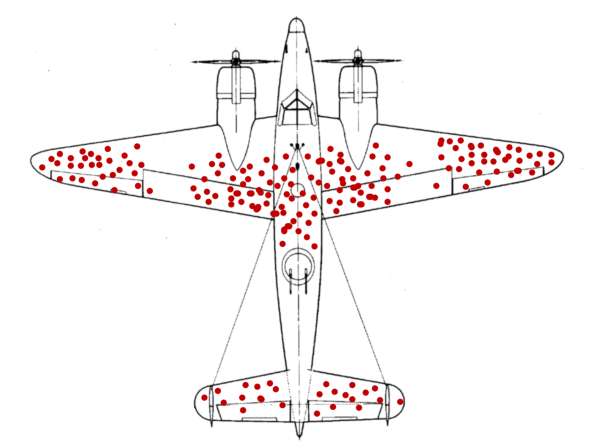
\includegraphics[width=0.6\textwidth]{c1.plane.01.png}
    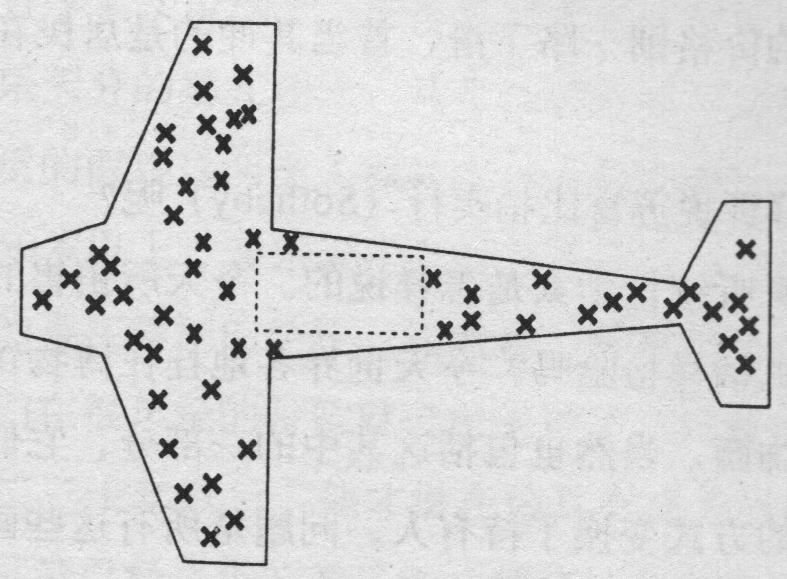
\includegraphics[width=0.6\textwidth]{c1.plane.04.png}
  \end{figure}
\end{frame}

\begin{frame}
  \frametitle{案例分析 | 幸存者偏见 | 天主教徒变成基督教徒}
  \begin{block}{近10年来美国大约有400万名天主教徒变成了基督教徒}
通过对全美基督教牧师的横截面展开调查,《基督教先驱报》得到了调查结果。调查共发出25000份问卷,其中2219名牧师反馈回了问卷。回收的问卷显示:在过去10年里共有51361名原罗马天主教徒变成了基督教徒。根据样本推算,得到了全国范围的估计:近10年来全美共有4144366名天主教徒改变信仰,变成了基督教徒。即便考虑到误差,全美范围内这一数据也不可能少于200万或者300万,而且很有可能接近500万。
  \end{block}
  \pause \pause \pause \pause
  \begin{block}{解析}
    被调查的牧师中超过90\%的人没有发表看法,或者他们中大多数都早已将调查问卷投进了纸篓。
  \end{block}
  \pause
  \begin{block}{可能的问题}
    《基督教先驱报》 vs. 基督教 vs. 天主教
  \end{block}
\end{frame}

\begin{frame}
  \frametitle{案例分析 | 幸存者偏见 | 耶鲁毕业生的年收入}
  \begin{block}{案例}
    1924级的耶鲁毕业生平均年收入为25111美元。
  \end{block}
  \pause \pause \pause \pause
  \begin{block}{疑点}
    \begin{itemize}
      \item 惊人的准确,竟然精确到以元为单位。
      \item 大得令人难以置信。
    \end{itemize}
  \end{block}
  \pause
  \begin{block}{解析}
    \begin{itemize}
      \item 很难知道非常准确的年收入
      \item 涉及收入——夸大(虚荣)与缩小(偷税漏税)
      \item 最大误差的可能来源:收入数据建立在能够取得联系并愿意回答问卷的耶鲁学生样本之上
    \end{itemize}
  \end{block}
\end{frame}

\begin{frame}
  \frametitle{案例分析 | 幸存者偏见 | 耶鲁毕业生的年收入}
  \begin{block}{25111美元的庐山真面目}
    \begin{itemize}
      \item 1924级耶鲁学生中能够联系上的
      \item 愿意站出来说出收入的
      \item 假定说的都是真话
    \end{itemize}
  \end{block}
  \pause
  \begin{block}{假定说真话}
    \begin{itemize}
      \item 了解杂志读者阅读量的上门调查,美国人每天刷牙1.02次
      \item 人们会说真话的假定往往是不可靠的,几乎所有的调查者都无法阻止人们往自己脸上贴金的做法。
    \end{itemize}
  \end{block}
\end{frame}

\begin{frame}
  \frametitle{案例分析 | 幸存者偏见 | 每个人都有点神经质}
  \begin{block}{心理医生的结论}
    一位心理医生曾经写道:实际上每个人都有点神经质。
  \end{block}
  \pause \pause \pause \pause
  \begin{block}{疑问}
    他观察了哪些人才得到了上述结论?
  \end{block}
  \pause
  \begin{block}{解析}
    \begin{itemize}
      \item 他是在对他的病人进行研究后才得到了这个发人深省的结论。
      \item 如果一个人心理健全,他是永远都不会接受心理医生的治疗的。
    \end{itemize}
  \end{block}
\end{frame}

\subsection{其他有偏抽样}
\begin{frame}
  \frametitle{案例分析 | 发表性偏见}
  \begin{block}{发表性偏见}
    \begin{itemize}
      \item 肯定性的研究发现相比否定性的研究发现来说,更有可能被发表,从而影响我们对事实真相的判断。
      \item 无论是医学还是其他领域,否定性的发现都显得单调乏味。这种发表性偏见将会导致研究结果的扭曲。
    \end{itemize}
  \end{block}
  \pause
  \begin{block}{抗抑郁药物药效发表性偏见}
    《纽约时报》曾发表了一篇关于抗抑郁药物药效发表性偏见的文章,第一句话就是:“抗抑郁药百忧解、帕罗西汀等产品的生产商故意不发表更多的药物试验结果,就是为了获得政府许可,误导医生和消费者对药物真实效果的看法。”那些证明这些药物对治疗抑郁症有效的研究中有94\%都得到了发表,而发现这些药物无效的研究中只有14\%被发表在相关刊物上。
  \end{block}
\end{frame}

\begin{frame}
  \frametitle{案例分析 | 记忆性偏见}
  \begin{block}{饮食习惯和癌症关系}
    1993年,一项关于饮食习惯和癌症关系的研究收集了两组女性的饮食习惯数据,一组对象为被诊断出患有乳腺癌的女性,另一组对象则由年龄相仿的健康女性组成,通过对她们早年的饮食习惯进行对比研究发现:患有乳腺癌的女性在年轻时喜欢吃高脂肪含量食物的人数明显偏多。
  \end{block}
  \pause \pause \pause \pause
  \begin{block}{解析}
    \begin{itemize}
      \item 这项研究并不能揭示饮食习惯和癌症之间的关系,仅仅只是告诉我们癌症是如何影响一个女人对她早期饮食习惯的记忆的。
      \item 患有乳腺癌的女性在回忆她们的饮食构成时,食物的脂肪含量明显上升了,甚至比她实际摄入的要高得多;而没有患上乳腺癌的女性则没有这一倾向。
    \end{itemize}
  \end{block}
\end{frame}

\begin{frame}
  \frametitle{案例分析 | 健康用户偏见}
   \begin{block}{思维实验}
     假设公共卫生官员发布一个理论:所有家长都应该给他们刚出生的孩子穿上紫色睡衣睡觉,因为这会刺激孩子的大脑发育。20年后,纵向研究证实,穿紫色睡衣睡觉的孩子更有可能在人生中获得成功:在哈佛大学学习的大一新生中,有高达90\%的人在孩童时期(甚至到现在)都穿着紫色睡衣入睡;而在马萨诸塞州州立监狱系统内的犯人中,只有3\%的人有穿紫色睡衣入睡的童年经历。
   \end{block} 
  \pause \pause \pause \pause
   \begin{block}{解析}
     \begin{itemize}
       \item 紫色睡衣当然不会有什么作用,真正起作用的是给他们的孩子穿上紫色睡衣的家长。
       \item 对于那些试图揭示某些活动(如定期运动或喝蔬菜汤等)是否对健康有益的研究来说,这样的一种偏见可能会使结论变得没有那么清晰。
     \end{itemize}
   \end{block}
\end{frame}

\begin{frame}
  \frametitle{案例分析 | 英国的刺猬量}
  \begin{block}{“路上哺乳动物调查”}
    2002年,刺猬调查扩大为“路上哺乳动物调查”。这项调查在每年的6-8月进行,正值哺乳动物迁移的时节,为了测量它们的活体数量,计算在柏油路上有多少压扁的残骸。
  \end{block}
  \pause \pause \pause \pause
  \begin{block}{解析}
    \begin{itemize}
      \item 这项调查算的到底是刺猬量还是车流量?
      \item 横死在路上的刺猬变少,会不会是它们随着环境进化,变聪明了?
      \item 也有可能是全球气候变迁,改变了刺猬的习性,让它们变得很少在那3个月中走在路上。
    \end{itemize}
  \end{block}
\end{frame}

\begin{frame}
  \frametitle{案例分析 | 其他案例}
  \begin{block}{有偏抽样}
    \begin{itemize}
      \item 针对大学生调查对于高中教育的看法
      \item 针对股票的行骗伎俩
      \item 长寿村的长寿秘诀
      \item 读书无用论(2010年第六次全国人口普查,大专以上文化程度的人口仅占总人口的8.7\%左右)
      \item 通过买彩票发家致富
      \item 投资购买古代或者现代的艺术品
      \item 全球的艾滋病病例数
      \item 海里的鱼量:科学家 vs. 渔民
      \item 在高铁上调查买到车票的比例
      \item 婴儿的身高、体重与头围生长曲线
    \end{itemize}
  \end{block}
\end{frame}

\begin{frame}
  \frametitle{案例分析 | 其他案例}
    \begin{figure}
      \centering
      
\includegraphics[width=0.45\textwidth]{c1.ticket.01.jpg}\quad
      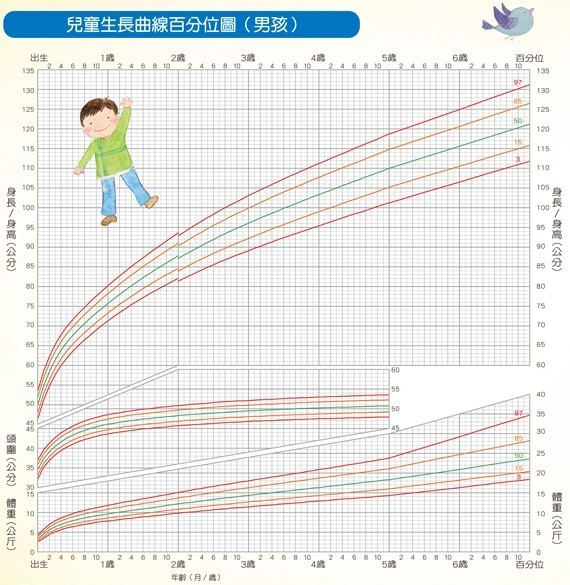
\includegraphics[width=0.4\textwidth]{c1.baby.01.jpg}
    \end{figure}
\end{frame}

\begin{frame}
  \frametitle{案例分析 | 其他案例}
  \begin{block}{有偏抽样}
    \begin{itemize}
      \item 美国民主党选民(女性更多)对性生活的满意程度比不上共和党的选民。
      \item 《超自然与占星师月刊》对读者调查表明70\%的英国人相信有神仙。
      \item 一项调查指出,新妈妈们平均花费400英镑在婴幼儿服装上。
      \item 不论男女,晚上饮用最多的饮料都是茶。
      \item 研究显示,有52\%的都市男性承认,一周至少会穿一次不成对的袜子(某家网络袜子零售商所做的调查)。
      \item 60\%的女性喜欢名人看起来有点小缺点,而76\%的英国男性则喜欢形象完美的名人(由某家化妆品公司及高画质电视频道所赞助的调查)。
      \item 英国有超过2000万的屋主,总共已经花费了1500亿英镑以上在没品位的居家改造上,以致降低了房屋的价值(由某家房地产保险公司好心告诉我们)。
    \end{itemize}
  \end{block}
\end{frame}

\section{知识拓展}
\begin{frame}
  \frametitle{知识拓展 | 德州神枪手谬误}
  \begin{block}{德州神枪手谬误}
    德州神枪手谬误(Texas sharpshooter fallacy),是一种因果谬误,原用以形容流行病学上的群集错觉,后衍伸泛指将统计上随机产生的群集独立出来,宣称有统计显著性的谬误。通俗地讲,就是在大量的数据/证据中刻意地挑选出对自己的观点有利的数据/证据,而将其余对自己不利的数据/证据弃之不用。\\
    \vspace{0.5em}
    德州神枪手谬误源自一个典故:有个德州人朝着自己的谷仓射了许多子弹,在弹孔最密集的地方画一个圈,然后自称是神枪手。
  \end{block}
  \pause
  \begin{block}{示例}
    在论证中国的国民生活水平时,仅仅只使用上海、广州、香港等发达都市的相关数据,或者仅仅只使用贵州、甘肃、青海等落后省份的相关数据。
  \end{block}
\end{frame}

\section{图说天下}
\begin{frame}
  \frametitle{图说天下 | 特朗普的推特——“双重人格”}
  \begin{figure}
    \centering
    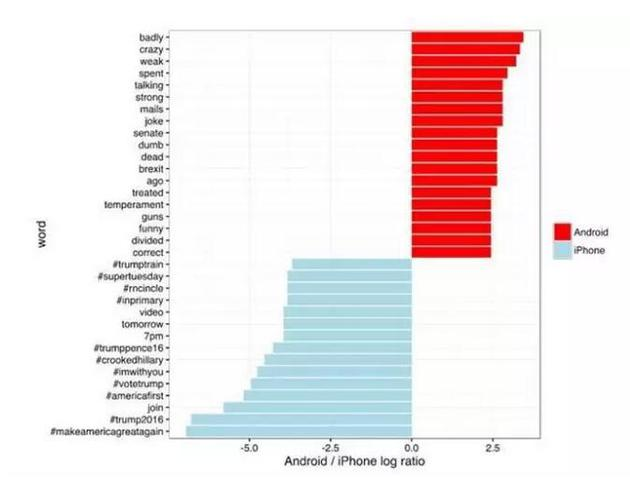
\includegraphics[width=0.85\textwidth]{c1.trump.01.jpg}
  \end{figure}
\end{frame}

\section{统计知识}
\begin{frame}
  \frametitle{统计知识 | 总体 vs. 样本}
  \begin{figure}
    \centering
    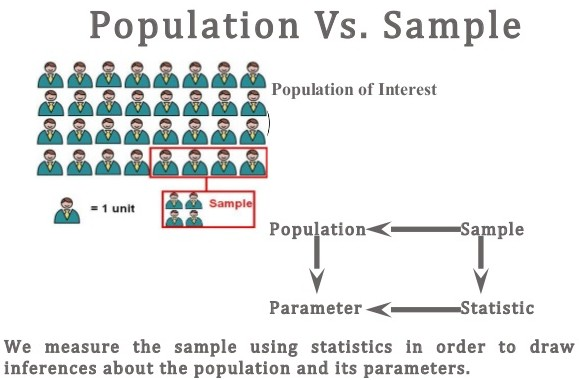
\includegraphics[width=0.5\textwidth]{c1.pvss.02.jpg}\\
    \vspace{0.5em}
    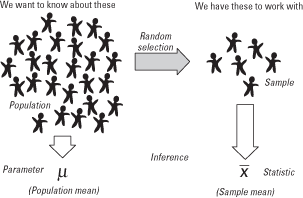
\includegraphics[width=0.45\textwidth]{c1.pvss.01.png}
  \end{figure}
\end{frame}

\begin{frame}
  \frametitle{统计知识 | 抽样方法}
  \begin{figure}
    \centering
    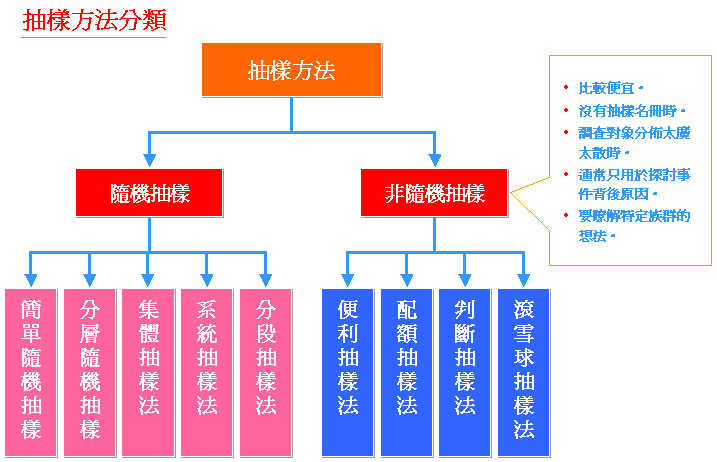
\includegraphics[width=0.5\textwidth]{c1.sm.01.png}\\
    \vspace{0.5em}
    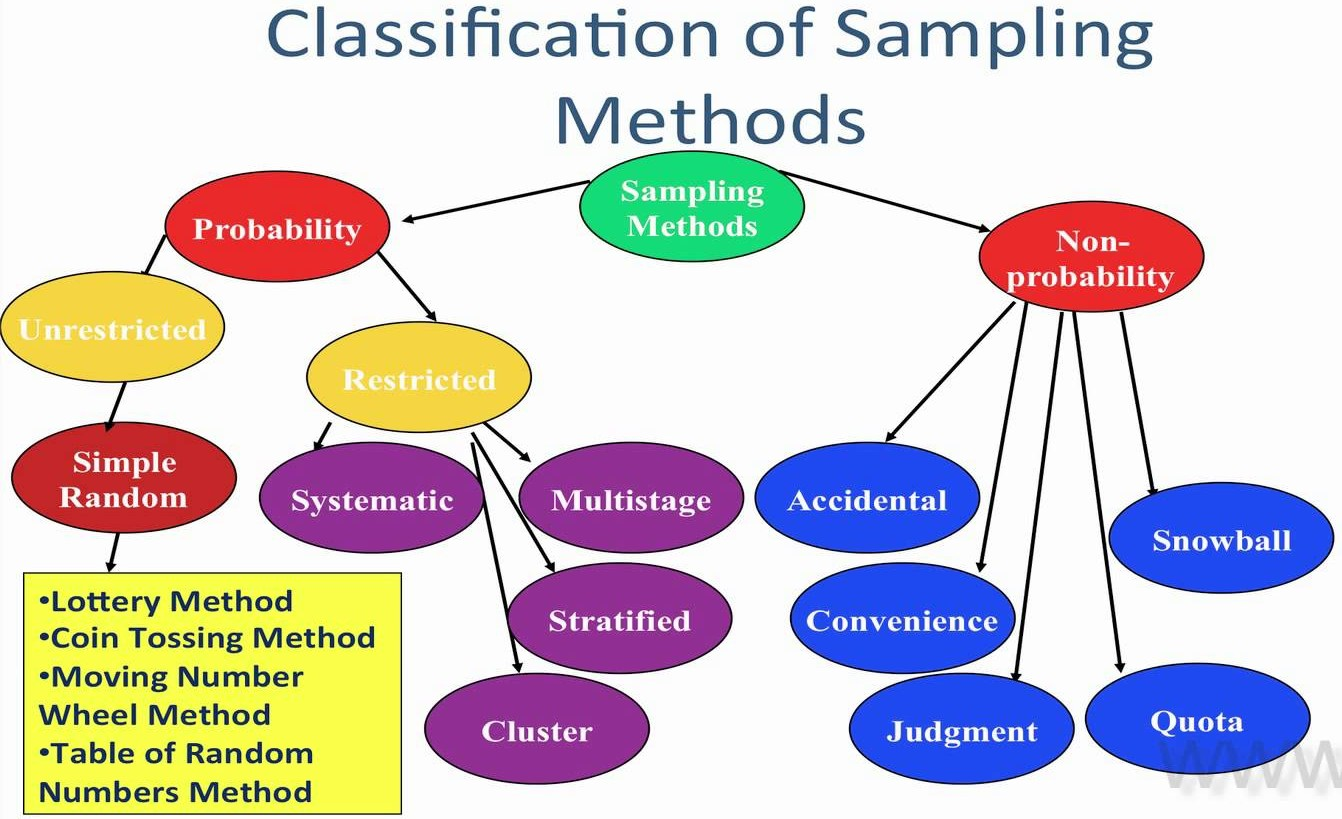
\includegraphics[width=0.5\textwidth]{c1.sm.02.jpg}
  \end{figure}
\end{frame}

\begin{frame}
  \frametitle{统计知识 | 抽样方法 | 举例}
  \begin{figure}
    \centering
    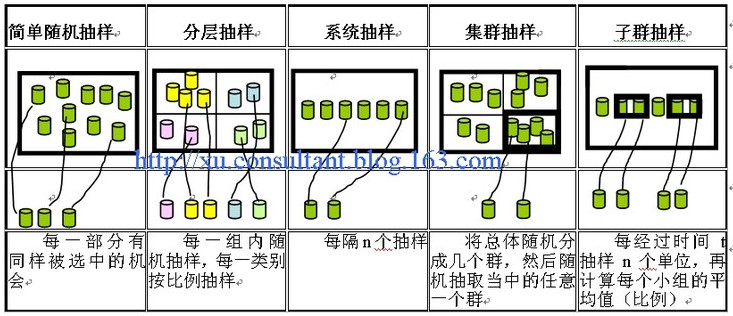
\includegraphics[width=0.7\textwidth]{c1.sme.02.jpg}\\
    \vspace{0.5em}
    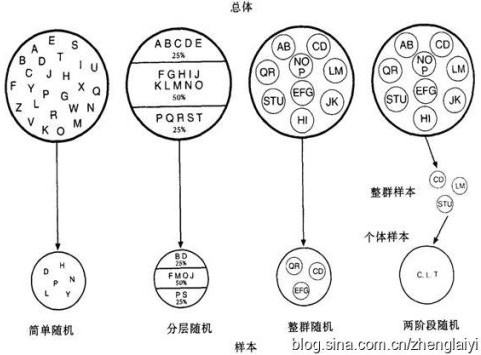
\includegraphics[width=0.45\textwidth]{c1.sme.01.jpg}
  \end{figure}
\end{frame}

\begin{frame}
  \frametitle{统计知识 | 抽样方法 | “失误” $\rightarrow$ 错误}
  \begin{figure}
    \centering
    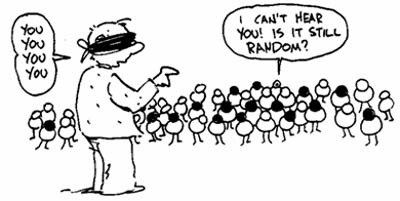
\includegraphics[width=0.6\textwidth]{c1.se.01.jpg}
  \end{figure}
  \pause
  \begin{block}{思考}
    《乡村教师》(刘慈欣)中的抽样
  \end{block}
\end{frame}

\begin{frame}
  \frametitle{统计知识 | 抽样方法 | 反面教材}
  \begin{figure}
    \centering
    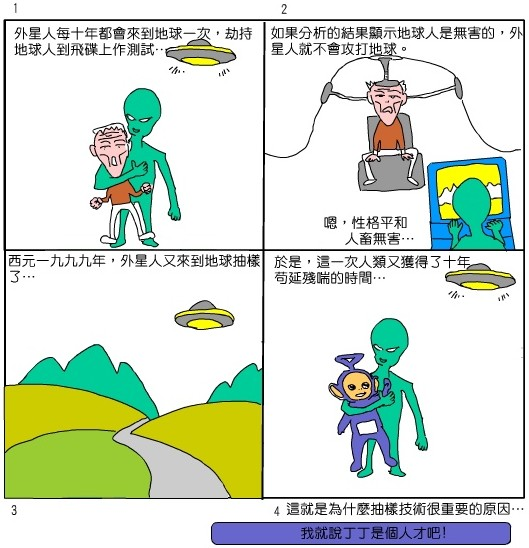
\includegraphics[width=0.6\textwidth]{c1.se.02.jpg}
  \end{figure}
\end{frame}

\begin{frame}
  \frametitle{统计知识 | 抽样方法 | 反面教材}
  \begin{figure}
    \centering
    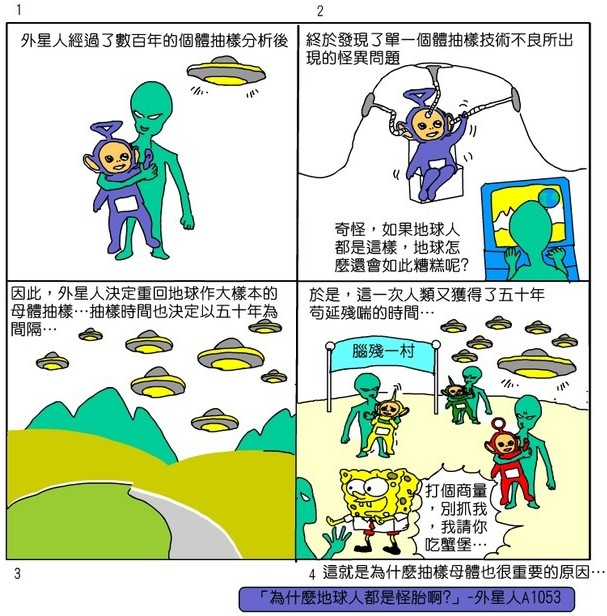
\includegraphics[width=0.6\textwidth]{c1.se.03.jpg}
  \end{figure}
\end{frame}

\begin{frame}
  \frametitle{统计知识 | 总结}
  \begin{itemize}
    \item 为了确保结论有价值,根据抽样得到的结论一定要采用具有代表性的样本,这种样本才能排除各种误差。
    \item 无形的误差与有形的误差一样容易破坏样本的可信度。也就是说,即使你找不到任何破坏性的误差来源,但只要有产生误差的可能性,你就有必要对结果保留一定的怀疑。
    \item 最基本的样本是随机样本,它是指完全遵循随机原则从总体中选出的样本。总体即形成样本的母体。 
    \item 随机样本的检验方法是:总体中的每个名字或每个事物是否具有相同的几率被选进样本?
    \item 纯随机样本是唯一有足够把握经受统计理论审查的样本。但它也有不足之处,在很多情况下,获得这种样本的难度很大并且十分昂贵,以至于单纯考虑成本就会排除它。
    \item 分层随机抽样是一个更经济的替代品,目前在民意调查和市场研究等领域中得到了广泛的应用。
    \item 一般而言,民意调查都带有一定程度的误差。
  \end{itemize}
\end{frame}



\section*{Acknowledgements}
\begin{frame}
  \frametitle{Powered by}
  \begin{center}
    
\includegraphics[width=9cm]{power.png}
  \end{center}
\end{frame}

\end{document}

